\documentclass[10pt, t,
aspectratio=169,% for widescreen (16:9) presentations
%aspectratio=1610,% for (16:10) presentations
%aspectratio=43,% for traditional (4:3) presentations
% handout%
usenames,
dvipsnames,
]{beamer}

\usetheme{Berkeley}
\usepackage{subcaption}
\usepackage{xcolor}
\usepackage{xspace}
\usepackage{algorithm}
\usepackage[noend]{algpseudocode}
\usepackage{listings}
\usepackage{tikz}
\usetikzlibrary{arrows,
	petri,
	topaths,
	calc,
	positioning,
	automata,
}
\usepackage{siunitx}
\usepackage{diagbox}
\usepackage{tikz-network}
\usepackage{bibentry}
\usepackage{amsmath}
\usepackage{booktabs}

\bibliographystyle{apalike}

% add the following two lines to your document to get bigger arrows
\usetikzlibrary{arrows.meta}
\tikzset{>={Latex[width=3mm,length=3mm]}}

\newcommand{\TODO}[1]{\noindent\textcolor{green}{\textbf{TODO:} #1}}
\DeclareMathOperator*{\argmin}{arg\,min}

\title[Mikroprozessor Architektur] % (optional, only for long titles)
{Implementierung eines Softcore-Mikroprozessor für FPGAs}
\author[] % (optional, for multiple authors)
{Gruppe 2}

\institute[] % (optional)
{
}
\date[] % (optional)
{06. April 2022}

\begin{document}
	\frame{\titlepage}
	\begin{frame}{Microcontroller}
		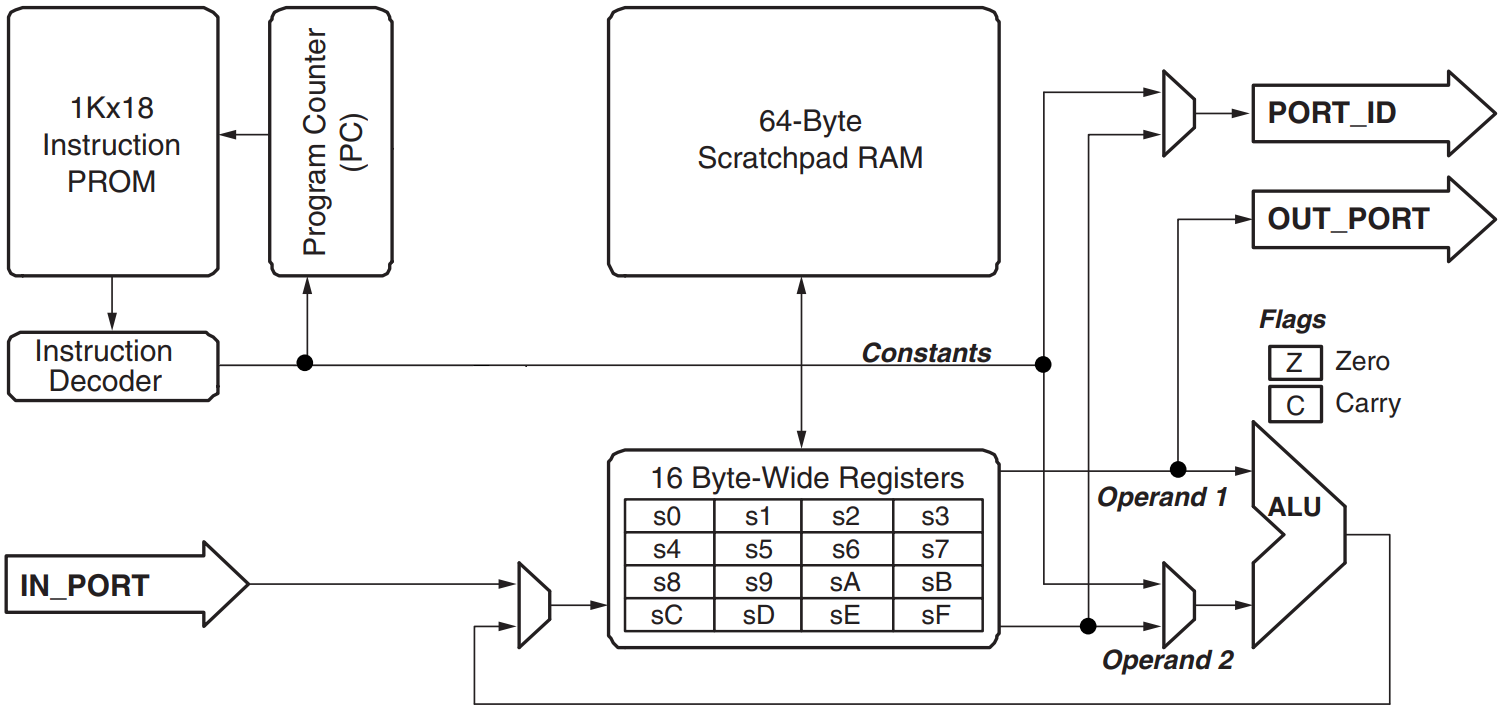
\includegraphics[width=.95\linewidth]{figures/Blockdiagram.png}
	\end{frame}
	\section{Betrachtete Befehle}
	\begin{frame}{Betrachtete Befehle}
		\begin{itemize}
			\item ADD-Befehl (z.B. ADD 17, 18)
			\item CALL-Befehl (z.B. CALL 23)
			\item STORE-Befehl (z.B. STORE 17, 42)
			\item OUTPUT-Befehl (z.B. OUTPUT 60, 240)
			\item Befehle benötigen 6 Taktzyklen, Sprünge (JUMP, CALL, RETURN) benötigen allerdings nur 4 Taktzyklen, da ALU, Register und Scratchpad RAM nicht benötigt werden
		\end{itemize}
	\end{frame}
	\section{ADD sX, sY}
	\begin{frame}{Instruction PROM}
		\begin{itemize}
			\item Befehl steht im Instruction PROM
			\item Program Counter gibt an, dass Befehl ausgeführt werden soll
			\item 18 bit Befehl wird an Instruction Decoder weitergegeben
			\\
			\includegraphics[width=1.0\linewidth]{figures/ProgramCounterBisInstructionDecoder.png}
		\end{itemize}
	\end{frame}
	\begin{frame}{Instruction Decoder}
		\begin{itemize}
			\item steuert Komponenten basierend auf der Instruktion an
			\item $\rightarrow$ Register soll sX und sY laden\\
			\item $\rightarrow$ ProgramCounter soll Adresse für nächsten Befehl bestimmen\\
			\item $\rightarrow$ MUX vor Register soll Ergebnis des Befehls wieder in Register sX speichern\\
			\item $\rightarrow$ ALU soll einen ADD sX, sY Befehl ausführen\\
			\item $\rightarrow$ MUX vor der ALU gibt den Wert aus dem Register an die ALU durch\\
		\end{itemize}
	\end{frame}
	\begin{frame}{Register}
		\begin{itemize}
			\item Register lädt Wert aus Registern sX und sY (Adressen in den Bits 11-8, 7-4) und gibt diese weiter
			\item MUX vor Register haben 3 Mögliche Input: \\
			\item $\rightarrow$ INPUT (extern) \\
			\item $\rightarrow$ ALU output \\
			\item $\rightarrow$ Scratchpad RAM output \\
			\item entscheiden, welcher Wert wieder in Register sX gespeichert wird
			\item bei Befehl ADD sX, sY: Output der ALU
			
		\end{itemize}
	\end{frame}

	\begin{frame}{Register}
		\includegraphics[width=1.0\linewidth]{figures/Register.png}
	\end{frame}
	
	\begin{frame}{ALU}
		\begin{itemize}
			\item Befehl wird Abhängig von Bits 17-12 ausgeführt, bei OP-Code 000000 ist das der Befehl ADD sX, sY
			\item MUX vor der ALU entscheidet, ob geladener Wert aus Register oder Immediate Wert von Instruction Decoder an ALU weitergegeben wird, bei ADD sX, sY: Wert aus Register
			\item Ergebnis der Berechnung wird an Register zurück gegeben
			\item Zero und Carry Bits werden gesetzt und an Instruction Decoder gegeben
		\end{itemize}
	\end{frame}
	
	\begin{frame}{Program Counter}
		\begin{itemize}
			\item Program Counter bestimmt Adresse des nächsten Befehls
			\item MUX vor Program Counter entscheidet, ob Adresse inkrementiert wird, oder ob man an eine spezielle Adresse springt
			\item $\rightarrow$ nach einem ADD sX, sY Befehl wird die Adresse einfach inkrementiert
			
		\end{itemize}
	\end{frame}

	\section{CALL aaa}

	\begin{frame}{Instruction Decoder}
		\begin{itemize}
			\item Call/Return Stack speichert Adresse des aktuellen Befehls auf den Stack
			\item MUX vor Program Counter bekommt vom Instruction Decoder Adresse aaa des nächsten Befehls
			\item MUX vor PC bekommt auch die Information, dass er Adresse aaa wählen soll
		\end{itemize}
	\end{frame}

	\section{STORE sX, ss}

	\begin{frame}{Instruction Decoder}
		\begin{itemize}
			\item Register soll Wert aus sX laden
			\item MUX vor ALU gibt Immediate Wert vom Instruction Decoder an Scratchpad RAM weiter
			\item Scratchpad RAM soll geladenen Wert an Adresse ss speichern
			\includegraphics[width=.4\linewidth]{figures/STORE.png}
		\end{itemize}
	\end{frame}

	\section{OUTPUT sX, pp}
	
	\begin{frame}{Instruction Decoder}
		\begin{itemize}
			\item MUX\_i\_o soll Port für Output bestimmen, \\ bei OUTPUT sX, pp: immediate Wert pp
			\item Register soll Wert von Adresse sX ausgeben
			\item Wert von Register wird an OUT\_PORT ausgegeben
			\item $\rightarrow$ bei Port 60 mit Wert 240 in Register sX wird eine rote LED auf dem Board auf nahezu maximale Helligkeit gestellt
		\end{itemize}
	\end{frame}
	
	\section{enable\_i}
	
	\begin{frame}{Enable Bits}
		\begin{itemize}
			\item Der Instruction Decoder setzt alle enable\_i-Bits der Komponenten, die im aktuellen Befehl nicht verwendet werden auf 0.
			\item $\rightarrow$ bei einem OUTPUT Befehl ist das write\_enable\_i Bit beim Register auf 0, da nur Werte gelesen werden etc.
			\item ist Grund, weshalb Befehle mehr als einen Taktzyklus brauchen
		\end{itemize}
	\end{frame}

	\begin{frame}{Microcontroller}
		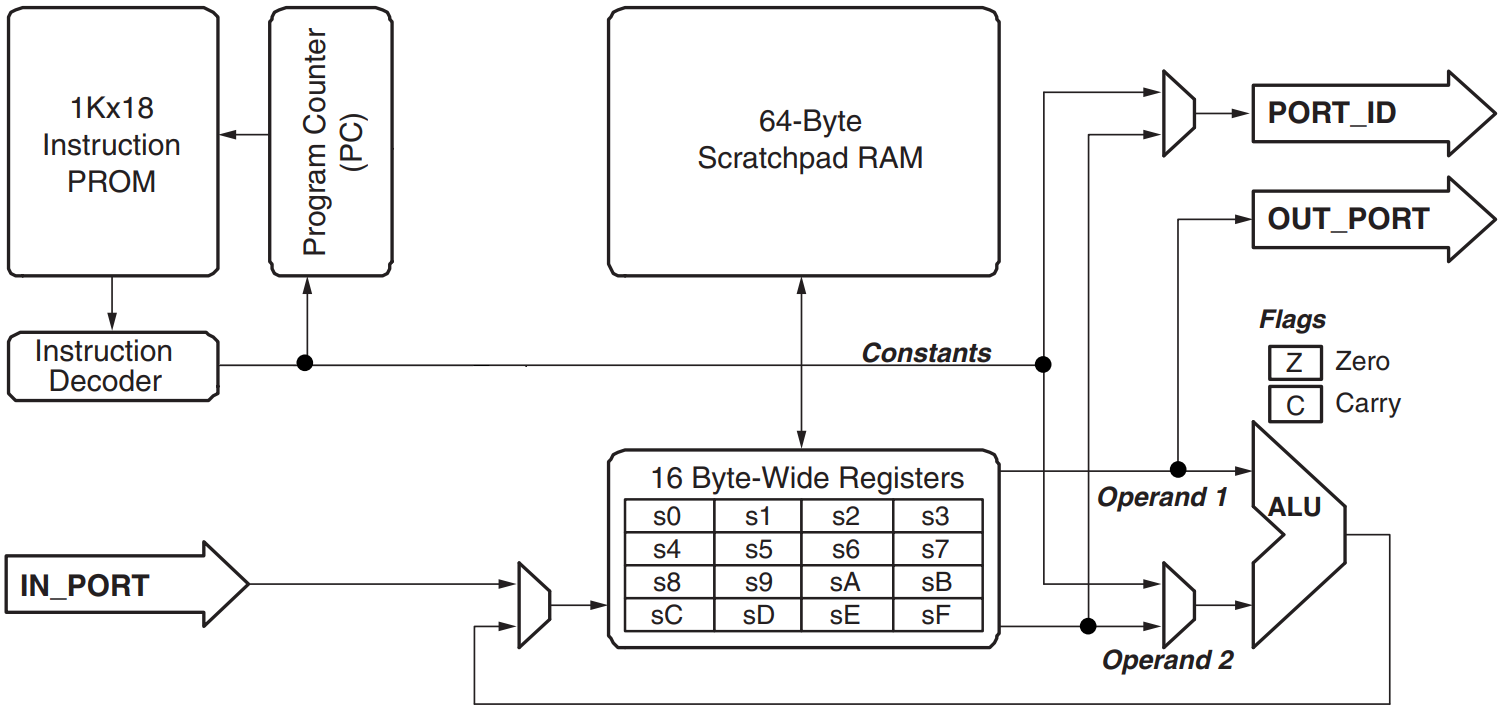
\includegraphics[width=.95\linewidth]{figures/Blockdiagram.png}
	\end{frame}

\end{document}
